\documentclass{article}
\usepackage{amsmath,amsfonts} %use special character
\usepackage{graphicx} %Inseting image
\usepackage{hyperref} %use for link
\usepackage{algorithm} %use for Mathmatical model
\usepackage{algpseudocode} %use seudocode define
%\usepackage{cite}
\usepackage[a4 paper]{geometry} %%use for paper size
\usepackage{paralist} %use paralist
\usepackage{verbatim} %use comment
\usepackage{polyglossia} %use for kalpurush.ttf supported
\usepackage{fontspec} 
\newfontface{\bn}{kalpurush.ttf} % used for bangla write



\title{Research paper about machine learning}
\author{Golden Order}
\date{28th july, 2024}
\begin{document}
\maketitle
\section{Group Member}
\begin{itemize}%hspace means horizontal space
    \item \hspace{.4cm}  Name: Alamin \hspace{2.2cm} ID:CSE2102023107
    \item \hspace{.5cm}Name: Md.Tuhin Alam \hspace{1cm}ID:CSE2102023013
\end{itemize}
% We have writen the entire project together..
\section{abstract}
This paper explores the use of [specific machine learning method] in [specific application]. We present a detailed analysis of the [method] approach, including its implementation, evaluation, and comparison with other existing methods. Our results demonstrate that [method] achieves superior performance in terms of [specific metrics], suggesting its potential for broader applications in [field].


\section{Introduction}
Machine learning has emerged as a critical tool in the field of \textbf{[field]}, enabling the development of intelligent systems that can [task]. This paper focuses on \textbf{[specific aspect]}, aiming to address the limitations of current approaches and propose a novel solution using [method].

Recent advancements in \textbf{[related area]} have led to significant improvements in [outcome]. However, challenges such as [challenge] remain, motivating the need for further research. Our approach leverages [key technique], which allows for [benefit].

The structure of this paper is as follows: Section 2 reviews related work, Section 3 describes the methodology, Section 4 presents the experimental setup and results, and Section 5 discusses the findings. Finally, Section 6 concludes the paper with future directions.

\section{Related Work}
The study of [related topic] has seen substantial progress in recent years. For instance, [Author et al., Year] proposed [method/technique], which improved [performance measure] by \textit{[percentage]} compared to [baseline].

Other significant contributions include [Author, Year], who introduced [alternative approach], and [Author , Year], who focused on [specific problem]. Despite these advancements, challenges such as \underline{[specific challenge]} persist, which this paper aims to address.

\section{Methodology}
Our proposed method is based on [core idea]. We begin by [brief overview of steps], followed by a detailed explanation of each step.

\subsection{Data Preprocessing}
The data used in this study was collected from [source]. We performed Preprocessing steps such as [step 1], [step 2], and [step 3] to ensure [data quality].

\subsection{Model Architecture}
The architecture of our model consists of [layers/components]. Figure illustrates the structure of the model.

\begin{figure}[h]
    \centering
    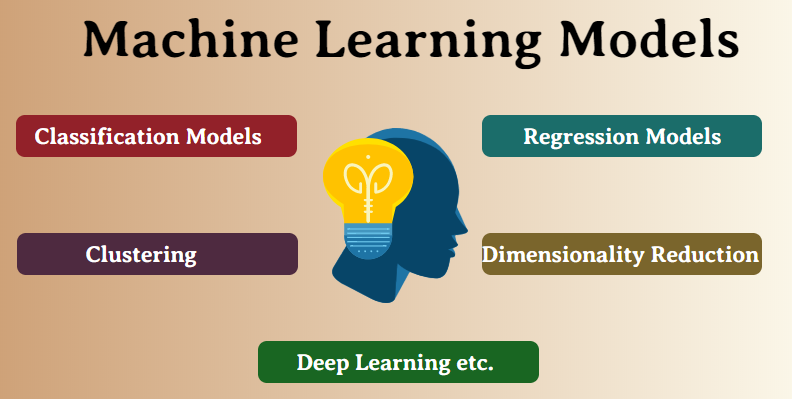
\includegraphics[width=0.8\textwidth]{2.png}
    \caption{Model architecture of the proposed method.}
    \label{fig:architecture}
\end{figure}

\subsection{Training Procedure}
We trained our model using [algorithm] with [hyperparameters]. The training process involved [number] epochs with a batch size of [size].

\begin{algorithm}
\caption{Training Algorithm}
\begin{algorithmic}[1]
\State Initialize parameters
\For{each epoch}
    \For{each batch}
        \State Compute loss
        \State Update parameters
    \EndFor
\EndFor
\end{algorithmic}
\end{algorithm}

\subsection{Evaluation Metrics}
To evaluate the performance of the model, we used [metrics], including [metric 1], [metric 2], and [metric 3]. These metrics provide a comprehensive assessment of [aspect] and allow for comparison with other methods.

\section{Experiments}
We conducted experiments on [dataset], which contains [number] samples of [data type]. The dataset was divided into training, validation, and test sets with [percentage] for each. The training dataset is 20\% and Validation or tasting is 80\%. 

\subsection{Baseline Comparison}
To validate our approach, we compared it against several baselines, including [baseline 1], [baseline 2], and [baseline 3]. Table shows the performance comparison.

\begin{table}[h]
\centering
\begin{tabular}{|c|c|c|c|}
\hline
Method & Metric 1 & Metric 2 & Metric 3 \\
\hline
Baseline 1 & X & Y & Z \\
Baseline 2 & A & B & C \\
Proposed Method & P & Q & R \\
\hline
\end{tabular}
\caption{Performance comparison of different methods.}
\label{tab:results}
\end{table}

\subsection{Ablation Study}
We performed an ablation study to analyze the impact of different components of our model. By systematically removing or altering [component], we observed [change in performance]. Figure illustrates the results.

\begin{figure}[h]
    \centering
    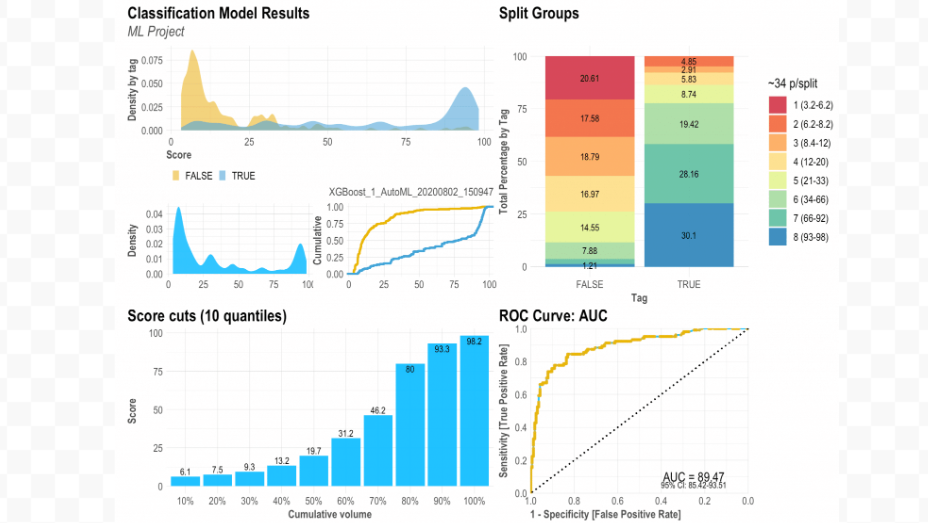
\includegraphics[width=0.8\textwidth]{1.png}
    \caption{Ablation study results.}
    \label{fig:ablation}
\end{figure}

\section{Results and Discussion}
Our experimental results demonstrate that [method] outperforms existing methods in terms of [metrics]. The improvement is particularly notable in [specific aspect], which can be attributed to [reason].

\subsection{Interpretation of Results}
The superior performance of our method suggests that [key insight]. This is further supported by [additional evidence or analysis], as shown in [figure/table].

\subsection{Limitations}
While our method shows promise, it has certain limitations, including [limitation 1] and [limitation 2]. Future work could address these by [suggestion].

\section{Conclusion}
In this paper, we presented a novel approach to [problem] using [method]. Our results indicate that this method offers significant advantages in terms of [benefit]. Future research could explore [future direction].\\
\copyright Goldern Order.. 

\section{\bn পেপার সংগ্রহ}
\bn আমরা পেপার লিখতে যার সাহায্য নিয়েছি 
 \cite{vartak2016modeldb}\\ 
\bibliographystyle{plain}

\bibliography{reference}
\end{document}
